\chapter{Requerimientos}
\section{Analisis de requerimientos}
�Cu\'al es la finalidad de esta actividad dentro de la empresa?
\\%
\\%
Garantizar que el Sistema Administre todos los procesos conferidos a los clientes.
\\%
\\%
�Qu\'e pasos se siguen para llevarla a cabo?
\\%
\\%
Software el cual llevara toda la administraci\'on de todas las opiniones quejas o cometarios.
\\%
\\%
�D\'onde se realizan estos pasos?
\\%
\\%
Los pasos se empiezan a realizar en las opiniones o dudas que tiene los clientes el cual hay un medio para que ellos puedan realizarlo de esta manera aqui es donde empezaremos a efectuar nuestro sistema CRM.
\\%
\\%
�Cu\'anto tiempo tardan en efectuarlos?
\\%
\\%
Al tener algun cometario de un cliente al efectuarse es en poco tiempo, ya que seria el tiempo de analisis de cometario realizado no mas de 10 minutos por cada cometario.
\\%
\\%
�Con cuanta frecuencia lo hacen?
\\%
\\%
La Gesti\'on de informaci\'on estar\'a actualizada siempre que se ingresen datos a los registros de informaci\'on de la organizacion esto permite tener un control inmediato de cualquier informaci\'on.
\\%
\\%
�Qui\'enes emplean la informaci\'on resultante?
\\%
\\%
Administrador del aplicativo el cual llevara el reporte diario de los movimientos y cometarios realizados por los clientes.%
\section{Analisis de requerimientos}
\subsection{Requerimientos generales}
\\%
\\%
�Qu\'e es lo que se hace?
\\%
\\%
Administrar un proceso el cual hace referencia a los comentarios, dudas, opinioes, quejas, etc, de los clientes y lo que se hace es cojer esta infromacion para poder tenerla en cuenta para la organizacion y tener presente toda esta informacion de cada cliente.
\\%
\\%
�C\'omo se hace?
\\%
\\%
Por medio de un software el cual esta adecuado para poder administrar estos procesos, ya que estes procesos tiene gran cantidad de datos por eso se requiere de un sistema que administre. y el mas adecuado es el CRM.
\\%
\\%
�Con que frecuencia se realiza?
\\%
\\%
Se realiza diariamente ya que es un sistema de administraci\'on de procesos y los procesos se est\'an efectuando diariamente, ya que en todo momento se estan efecutando comentarios de los clientes.
\\%
\\%
�Cu\'al es el grado de eficiencia con el que se efect\'uan las tareas?
\\%
\\%
Definir\'iamos como alta aunque quedar\'ia muy robusto por la calidad de datos que ingresara cada departamento de la organizaci\'on y su base de datos la cual se actualizara con cada informaci\'on nueva obtenida. El software tendr\'a un alto desempe�o con espuestas inmediatas y f\'acil control de consultas.
\\%
\\%
\subsection{Requerimientos b\'asicos}
�Cu\'al es el proceso b\'asico de la empresa?
\\%
\\%
El proceso b\'asico de la empresa es la producci\'on para el cual implementaremos el software de administraci\'on de procesos.
\\%
\\%
�Qu\'e controles de desempe\~no utiliza?
\\%
\\%
Seguimiento diario por el administrador. El cual observara  los procesos de la organizacion y de la misma forma  el funcionamiento del software.
\section{Requerimientos funcionales}
\begin{figure}[htbp]
%centering es para centrar la imagen
	\centering
%aca es donde se incluye la imagen, se da el ancho(width), \textwidth significa que con repescto al tamano del
%texto y luego la ruta, relativa siempre es decir, a partir de donde se esta, como images esta ahi
%dentro, solo se usa desde images y ojala nada de espacios en el nombre de la imagen
		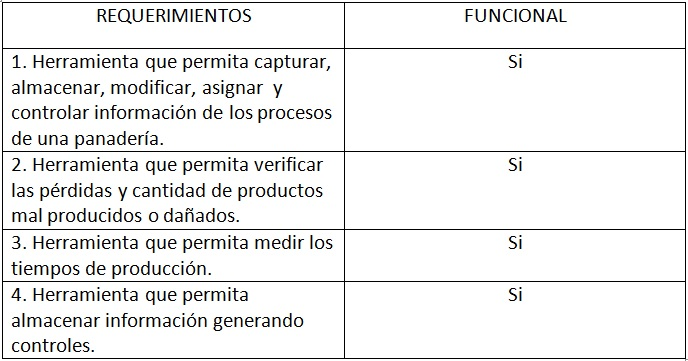
\includegraphics[width=0.60\textwidth]{images/requerimientosfuncionales.jpg}
%el caption es para el texto que aparece debajo de la imagen
	\caption{Requerimientos funcionales}
%label es para darle una referencia, por ejemplo si uno dice "como se puede ver en la imagen a1"
	\label{fig:Requerimientos funcionales}
\end{figure}%
\begin{figure}[htbp]
%centering es para centrar la imagen
	\centering
%aca es donde se incluye la imagen, se da el ancho(width), \textwidth significa que con repescto al tamano del
%texto y luego la ruta, relativa siempre es decir, a partir de donde se esta, como images esta ahi
%dentro, solo se usa desde images y ojala nada de espacios en el nombre de la imagen
		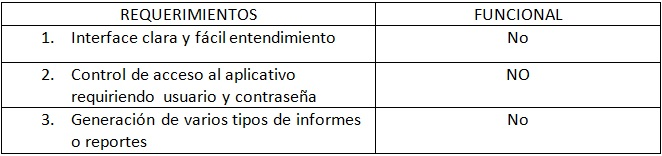
\includegraphics[width=0.60\textwidth]{images/requerimientosnofuncionales.jpg}
%el caption es para el texto que aparece debajo de la imagen
	\caption{Requerimientos no funcionales}
%label es para darle una referencia, por ejemplo si uno dice "como se puede ver en la imagen a1"
	\label{fig:Requerimientos no funcionales}
\end{figure}%

\begin{figure}[htbp]
%centering es para centrar la imagen
	\centering
%aca es donde se incluye la imagen, se da el ancho(width), \textwidth significa que con repescto al tamano del
%texto y luego la ruta, relativa siempre es decir, a partir de donde se esta, como images esta ahi
%dentro, solo se usa desde images y ojala nada de espacios en el nombre de la imagen
		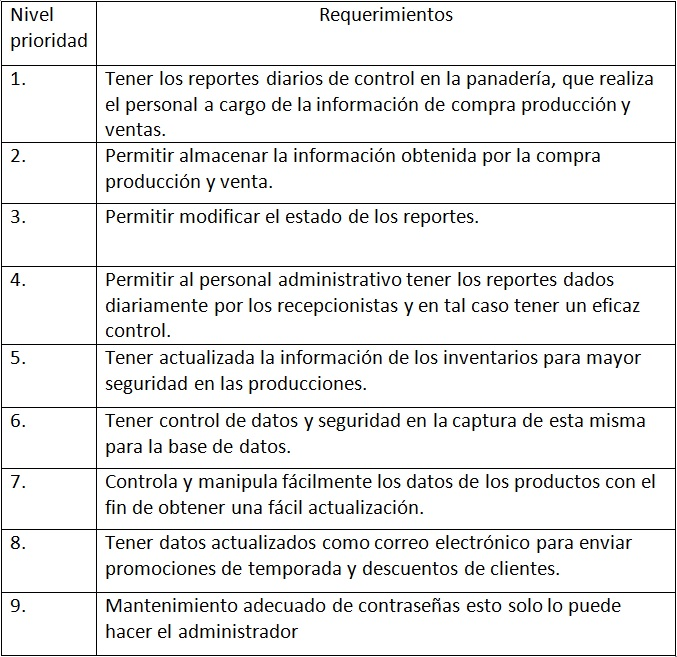
\includegraphics[width=0.60\textwidth]{images/requerimientos.jpg}
%el caption es para el texto que aparece debajo de la imagen
	\caption{Requerimientos}
%label es para darle una referencia, por ejemplo si uno dice "como se puede ver en la imagen a1"
	\label{fig:Requerimientos}
\end{figure}%
